\documentclass{utap}

\usepackage{wrapfig}
\usepackage{verbatim}
\usepackage{fancyvrb}
\usepackage{lscape}
\usepackage{rotating}
\usepackage{xepersian}

\title{تمرین شمارهٔ ۳}
\author{رامتین خسروی، \href{mailto:hadi.safari@ut.ac.ir?subject=[AP\%20S98 A3]\%20}{هادی صفری} و \href{mailto:ys.jafari@ut.ac.ir?subject=[AP\%20S98 A3]\%20}{یاسمن جعفری}}
\course{برنامه‌سازی پیشرفته}
\lecturer{رامتین خسروی}
\deadline{شنبه ۱۸ اسفند ۱۳۹۷، ساعت ۲۳:۵۵}
\graphicspath{{./img/}}
\renewcommand{\labelitemi}{$\circ$}
\renewcommand{\labelitemii}{$\diamond$}

\lstdefinelanguage{diff}{
    morecomment=[f][\color{Black}]{---},
    morecomment=[f][\color{Red}]<,
    morecomment=[f][\color{Green}]>,
    identifierstyle=\color{Cyan},
    basicstyle=\small\ttfamily\color{Cyan},
}

\begin{document}
    \maketitle

    \section{مصورساز برنامه}

    یکی از وظایف معاونت آموزشی و ادارهٔ آموزش در دانشگاه‌ها برنامه‌ریزی دروس است. این برنامه‌ریزی کاری پیچیده و دشوار است؛ زیرا باید وقت‌های خالی استادان، وجود فضای آموزشی مناسب، عدم تداخل کلاس‌هایی که دانشجویان ترم‌های مختلف رشته‌های گوناگون قصد دارند در آن‌ها شرکت کنند، استفادهٔ مفید از ساعات پربازده روز و چندین مؤلفهٔ دیگر در آن در نظر گرفته شود.

    معاونت آموزشی دانشکدهٔ برق و کامپیوتر دانشگاه تهران برای تسهیل برنامه‌ریزی چند ابزار کمکی را توسعه داده است که برخی اطلاعات مورد نیاز را مصور\footnote{\textit{مصورسازی داده} یا \lr{data visualisation} شاخه‌ای از آمار توصیفی است که به بررسی نحوهٔ نمایش تصویری داده‌ها می‌پردازد. در دنیای امروز و با اهمیت~یافتن کلان‌داده‌ها، نقش مصورسازی بسیار پراهمیت شده است.} می‌کند. یکی از این ابزارها مصورساز برنامه است که اطلاعات دروس ارائه‌شده را روی برنامهٔ هفتگی دانشکده نشان می‌دهد.

    \begin{figure}[hb]
        \centering
        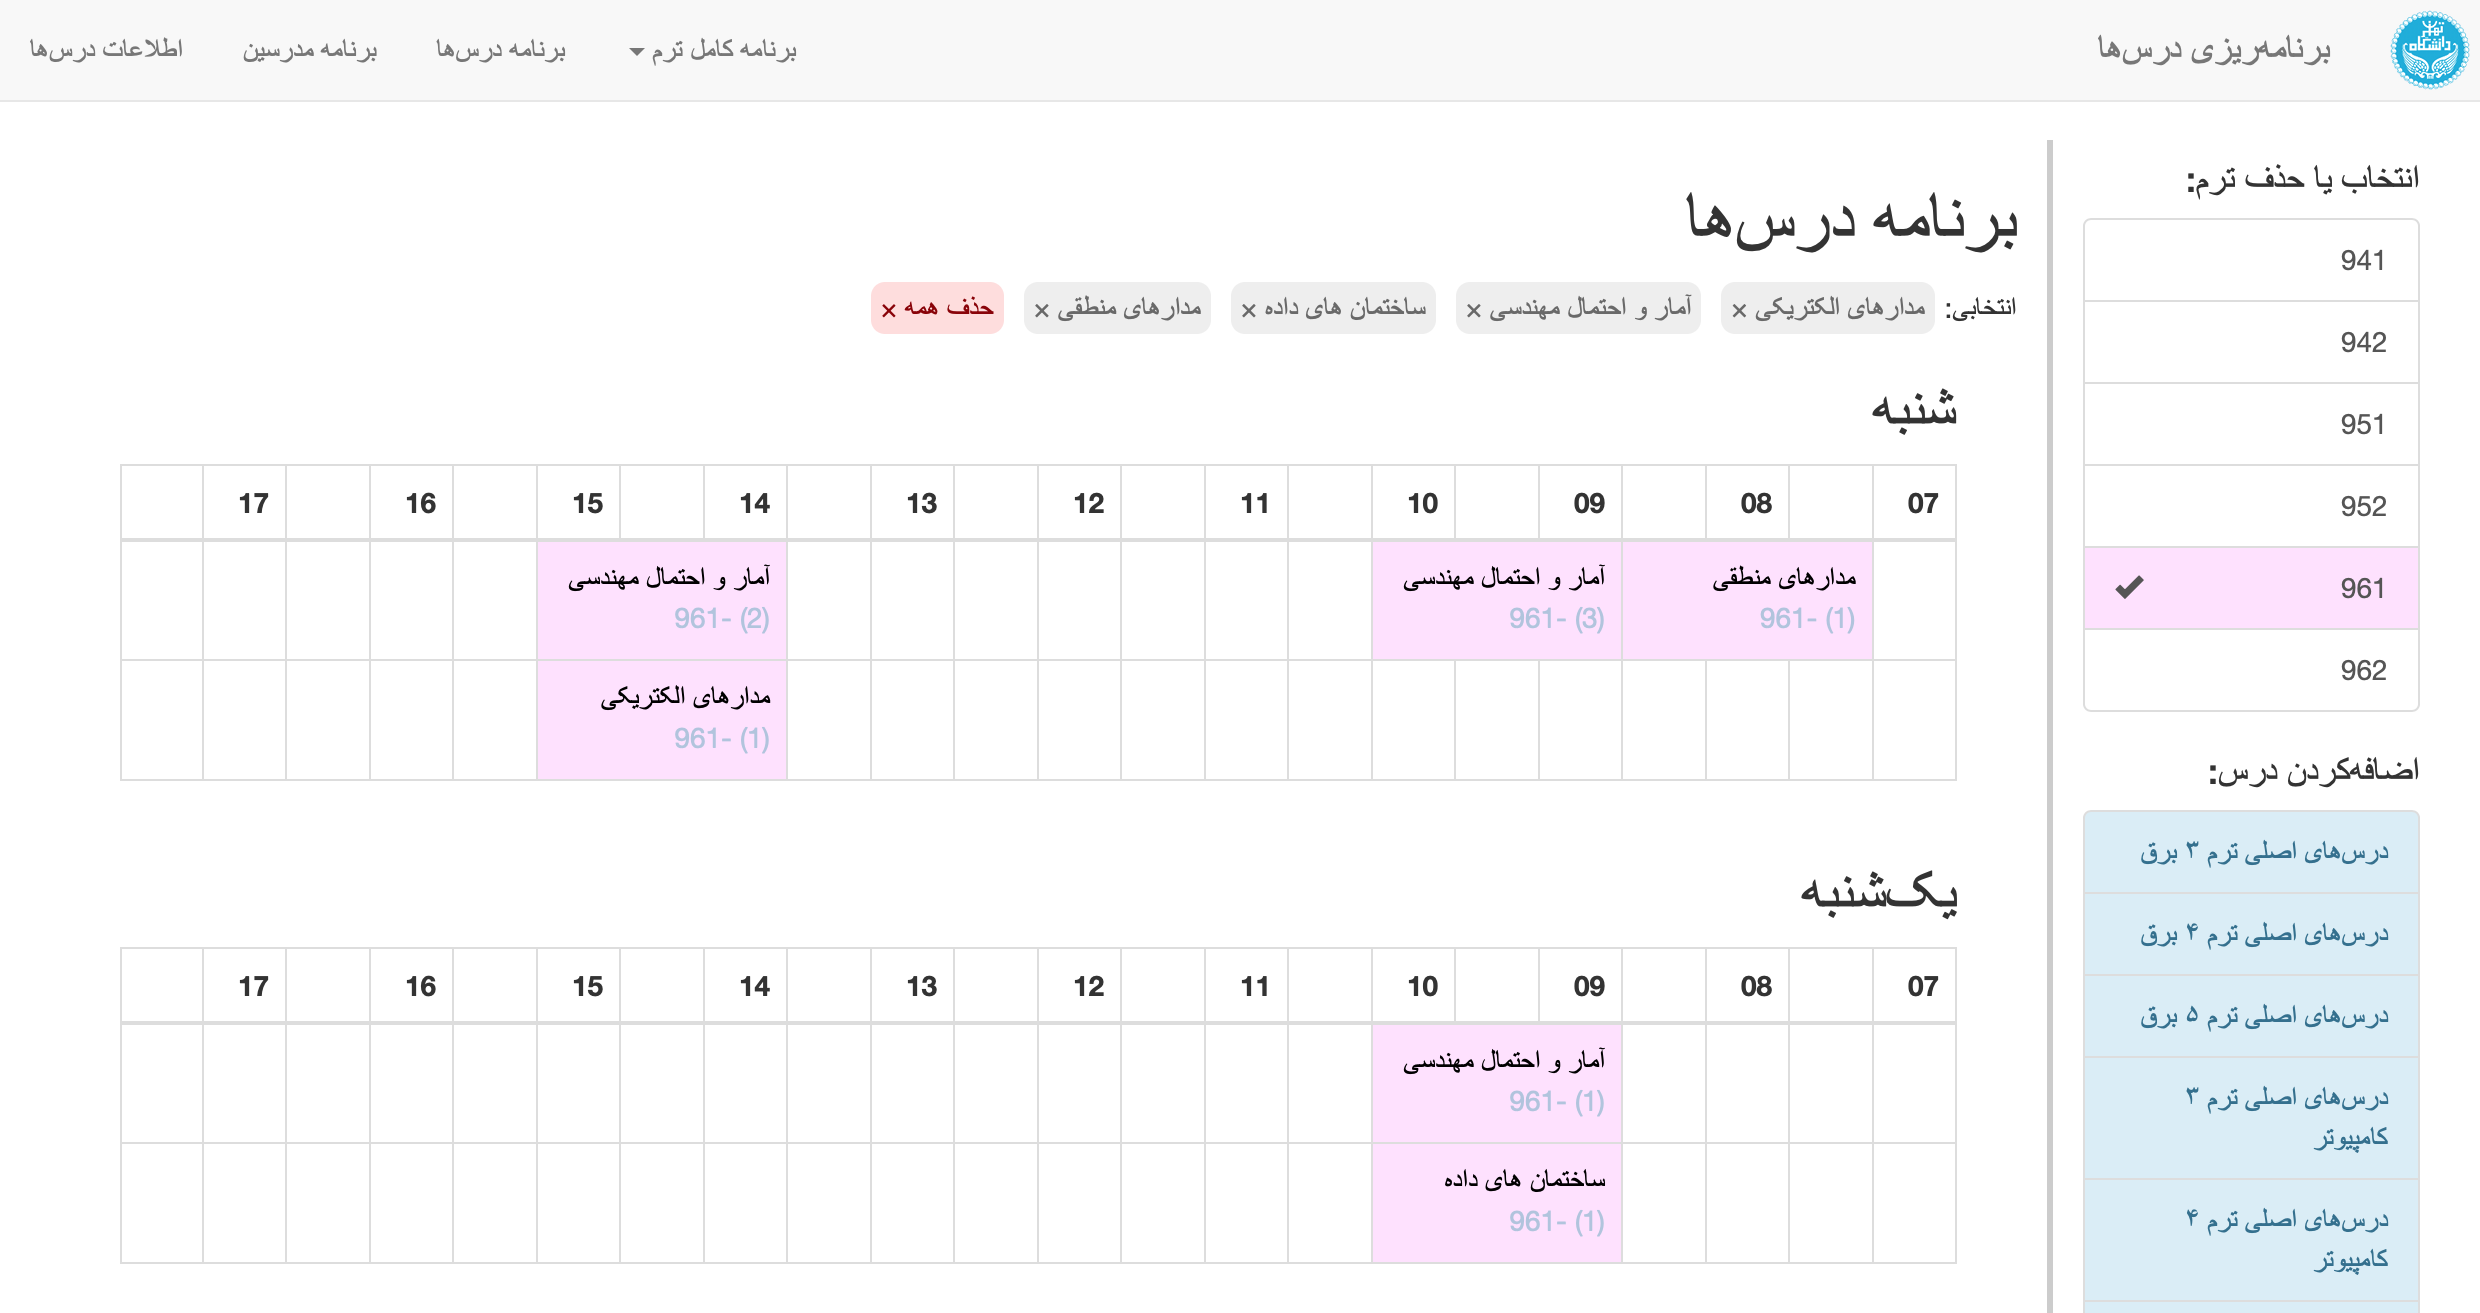
\includegraphics[width=0.7\textwidth]{webversion.png}
        \caption{مصورساز برنامه}
    \end{figure}

    با توجه به افزایش تعداد ورودی‌های رشته‌های مختلف دانشگاه که به پیچیده‌تر شدن فرآیند برنامه‌ریزی آموزشی منجر شده است، تصمیم بر این شد که نسخه‌ای از این برنامه به زبان \lr{C++} پیاده‌سازی شود تا بازدهی بالاتری داشته باشد و بتوان به‌سرعت انواع برنامه‌های رشته‌های مختلف را با آن مصورسازی کرد.

    \subsection{نحوهٔ عملکرد برنامه}

    ابتدا فهرستی شامل نام انگلیسی دروس دانشکده بر اساس شناسهٔ درس‌ها در اختیار برنامه قرار می‌گیرد. سپس اطلاعات ارائهٔ درس‌هایی که قرار است مصور شوند به برنامه داده می‌شوند.

    از هر درس ممکن است چندین گروه متفاوت ارائه شود و هر گروه از هر درس ممکن است چند بازهٔ زمانی در طول هفته را به خود اختصاص دهد. مثلاً درس آمار و احتمال مهندسی (با شناسهٔ 8101092) در ترم پاییز ۹۶ در سه گروه ارائه شده است. کلاس‌های گروه 03 را دکتر بهرک در ساعت‌های ۰۹:۰۰ تا ۱۰:۳۰ روزهای شنبه و ۰۹:۰۰ تا ۱۰:۳۰ روزهای دوشنبه برگزار کرده است.

    مصورساز ابتدا باید برای هر بازهٔ زمانی هر گروه درسی مکان مناسب را بیابد. ممکن است در یک زمان چندین کلاس درس در دانشکده برگزار شود؛ در نتیجه، گاهی نمایش همهٔ گروه‌های درسی در یک ردیف ممکن نیست. مصورساز برای یافتن مکان مناسب یک بازهٔ زمانی، آن را از پایین‌ترین ردیف به برنامهٔ یک روز هفته وارد می‌کند و تا جایی بالا می‌برد که با هیچ بازهٔ زمانی مربوط به گروه درسی دیگری برخورد نکند. اگر پایین‌ترین ردیف روز مورد نظر در آن بازهٔ زمانی پر بود، ردیف جدیدی به پایین آن روز اضافه می‌شود. برای فهم دقیق‌تر نحوهٔ چینش بازه‌‌های زمانی \nameref{sec:sample} را بررسی کنید. توجه کنید که نحوهٔ چینش بازه‌های زمانی با روش بیان‌شده برای هر ورودی یکتا خواهد بود و انتظار می‌رود برنامهٔ شما دقیقاً خروجی مورد انتظار را تولید کند.

    در انتها، مصورساز برنامهٔ هر هفته را بر اساس چینش تعیین‌شده به~شکل متنی تهیه می‌کند. نام انگلیسی درس بر اساس شناسهٔ درس استخراج می‌شود و در برنامهٔ هفتگی نمایش داده می‌شود.

    \subsection{قالب ورودی‌ها}

    ورودی‌های برنامه از سه بخش تشکیل می‌شود:

    \subsubsection{فهرست نام دروس}

    فهرستی از نام انگلیسی دروس بر اساس شناسهٔ  درس‌ها در پرونده‌ای با قالب \lr{CSV}\footnote{\textit{مقادیر جداشده با ویرگول} یا \lr{Comma-Separated Values} یک قالب رایج برای پرونده‌های متنی است که در آن مقادیر با استفاده از حائل کامای انگلیسی (\lr{\texttt{,}} با شناسهٔ \lr{ASCII} 44 یا \lr{0x2C}) از یکدیگر جدا می‌شوند. این پرونده‌ها را می‌توان با نرم‌افزارهای صفحه‌گسترده‌ای مانند \lr{Microsoft Excel}، \lr{LibreOffice Calc} یا \lr{Apple Numbers} مشاهده و ویرایش کرد.} ساده‌شده در اختیار برنامهٔ شما قرار می‌گیرد.

    در خط اول این پرونده، عبارت \lr{\texttt{id,alias}} درج شده است.

    در هر یک از خطوط بعدی، ابتدا شناسهٔ یک درس که یک عددی ۷‌رقمی است می‌آید و سپس بلافاصله بعد از یک ویرگول انگلیسی، نام انگلیسی آن درس ذکر می‌شود. تضمین می‌شود نام درس شامل فاصله\LTRfootnote{space} یا هر نویسهٔ فضای خالی\LTRfootnote{whitespace} دیگری نخواهد بود. برای مثال، یکی از خطوط بعدی ممکن است به شکل \lr{\texttt{8101119,adv-prog}} باشد که درس برنامه‌نویسی پیشرفته را نشان می‌دهد.

    آدرس این پرونده را به~عنوان آرگومان اول خط فرمان به برنامهٔ شما داده خواهد شد. برای آشنایی با نحوهٔ استفاده از آرگومان‌های خط فرمان به ضمیمهٔ~\nameref{sec:commandline-args} مراجعه کنید.

    \subsubsection{فهرست ارائه‌ها}

    فهرست گروه‌های مختلف درس‌هایی که باید مصور شوند از طریق ورودی استاندارد \lr{stdin} در اختیار برنامه گذاشته می‌شود.

    هر خط ورودی شامل بخش‌های زیر می‌شود که با نویسهٔ\LTRfootnote{character} فاصله (با شناسهٔ \lr{ASCII} ۳۲ یا \lr{0x20}) از هم جدا می‌شوند:
    \begin{description}[leftmargin=9em,style=nextline,font=\labelitemi\quad\bfseries]
        \item[شناسهٔ ارائه] شناسهٔ ارائه به‌ترتیب از شناسهٔ درس (یک عدد ۷‌رقمی) و شناسهٔ گروه (یک عدد ۲‌رقمی) تشکیل می‌شود که با نویسهٔ خط (\verb|-| با شناسهٔ \lr{ASCII} ۴۵ یا \lr{0x2D}) از هم جدا شده‌اند.
        \item[بازه‌های زمانی ارائه] هر ارائه یک یا چند بازهٔ زمانی را به خود اختصاص می‌دهد. بازه‌های زمانی با فاصله از هم جدا می‌شوند. هر کدام از بازه‌های زمانی ساختار زیر را دارند و اجزای آن‌ها با فاصله از هم جدا می‌شوند:
        \begin{description}[leftmargin=4em,style=nextline,font=\labelitemii\quad\bfseries]
            \item[روز] یکی از مقادیر \lr{\texttt{SAT}}، \lr{\texttt{SUN}}، \lr{\texttt{MON}}، \lr{\texttt{TUE}}، \lr{\texttt{WED}}، \lr{\texttt{THU}} یا \lr{\texttt{FRI}}
            \item[زمان] شامل زمان شروع و پایان که با نویسهٔ خط از هم جدا شده‌اند و هر یک از قالب \lr{\texttt{hh:mm}} تبعیت می‌کنند. دقیقه (\lr{\texttt{mm}}) یکی از دو مقدار \lr{\texttt{00}} یا \lr{\texttt{30}} را دارد و ساعت (\lr{\texttt{hh}}) با یکی از مقادیر \lr{\texttt{07}} تا \lr{\texttt{20}} مشخص می‌شود؛ بنابراین هر یک از زمان‌های شروع و پایان از ۵ نویسه تشکیل می‌شود. جداکنندهٔ ساعت و دقیقه نویسهٔ دونقطه (\lr{\texttt{:}} با شناسهٔ \lr{ASCII} ۵۸ یا \lr{0x3A}) است.
        \end{description}
    \end{description}

    مثلاً  یک خط ورودی که یک ارائهٔ درس برنامه‌نویسی پیشرفته را در ساعات ۱۰:۳۰ تا ۱۲:۰۰ روزهای یکشنبه و سه‌شنبه مشخص می‌کند ممکن است به شکل \lr{\texttt{8101119-01 SUN 10:30-12:00 TUE 10:30-12:00}} باشد.

    \subsubsection{عنوان برنامه}

    عنوان برنامه به~عنوان آرگومان دوم خط فرمان به برنامه داده می‌شود.

    \subsection{قالب خروجی‌ها}

    خروجی از چندین بخش تشکیل می‌شود:

    \subsubsection{عنوان}

    در ابتدای خروجی عنوان برنامه با پیشوند \lr{\texttt{\# }} نمایش داده می‌شود؛ مثلاً  ممکن است \lr{\texttt{\# Prog}} سطر اول خروجی را تشکیل دهد. بعد از این سطر یک سطر خالی نمایش داده می‌شود.

    \subsubsection{نام روز هفته}

    بعد از عنوان، برای هر یک از روزهای هفته نام روز با پیشوند \lr{\texttt{\#\# }} نمایش داده می‌شود؛ مثلاً  ممکن است \lr{\texttt{\#\# Saturday}} سطر بعدی خروجی را تشکیل دهد.

    نام روز به‌ترتیب یکی از عبارات \lr{\texttt{Saturday}}، \lr{\texttt{Sunday}}، \lr{\texttt{Monday}}، \lr{\texttt{Tuesday}}، \lr{\texttt{Wednesday}}، \lr{\texttt{Thursday}} یا \lr{\texttt{Friday}} خواهد بود. بعد از این سطر یک سطر خالی نمایش داده می‌شود.

    \subsubsection{خط زمان}

    در ادامه در یک خط زمان‌ها با قالبی شبیه ورودی (\lr{\texttt{hh:mm}}) می‌آیند. هر یک از ۲۸ بلوک مربوط به زمان‌ها به اندازهٔ ۱۰ شناسه طول دارد. زمان در سمت چپ ظاهر می‌شود و ادامهٔ  بلوک با نویسهٔ فاصله پر می‌شود. بلوک آخر استثنا حساب می‌شود و فقط به اندازهٔ  طول برچسب بلوک (۵ شناسه) طول خواهد داشت.

    در خط بعد به اندازهٔ مجموع طول بلوک‌ها نویسهٔ زیرخط (\lr{\texttt{\_}} با شناسهٔ \lr{ASCII} ۹۵ یا \lr{0x5F}) ظاهر خواهد شد.

    \subsubsection{بازه‌های زمانی ارائه‌ها}

    در خطوط بعدی، ردیف‌های مربوط به بازه‌های زمانی ارائه‌ها قرار می‌گیرد.
    
    هر ردیف از بازه‌های زمانی در سه سطر نمایش می‌یابد. سطر اول و سوم به حاشیه‌های افقی و گوشه‌ها اختصاص دارد و در سطر دوم حاشیه‌های عمودی و نام درس نمایش می‌یابد. حاشیه‌های افقی با نویسهٔ خط، حاشیه‌های عمودی با نویسهٔ خط عمودی (\lr{\texttt{|}} با شناسهٔ \lr{ASCII} ۱۲۴ یا \lr{0x7C}) و گوشه‌ها با نویسهٔ مثبت (\lr{\texttt{+}} با شناسهٔ \lr{ASCII} ۴۳ یا \lr{0x2B}) نمایش داده می‌شوند.
    
    هر بلوک زمانی در این خطوط طولی برابر ۱۰ نویسه دارد و از ستون زیر جداکنندهٔ ساعت و دقیقهٔ (\lr{\texttt{:}}) همان زمان آغاز می‌شود و تا ستون قبل از جداکنندهٔ ساعت و دقیقهٔ زمان بعدی ادامه می‌یابد. حاشیه‌های عمودی هر بازهٔ زمانی در اولین ستون اولین بلوک و آخرین ستون آخرین بلوک آن قرار می‌گیرند. بنابراین، در ابتدای همهٔ سطرهای مربوط به نمایش بازه‌های زمانی حداقل دو نویسهٔ فاصله قرار خواهد گرفت.

    بعد از آخرین بازهٔ زمانی هر ردیف چیزی نمایش داده نمی‌شود.

    هیچ سطر خالی‌ای از بازه‌های زمانی نمایش داده نمی‌شود.

    در انتهای خروجی هر روز هفته یک سطر خالی نمایش داده می‌شود.

    \subsubsection{نام درس}
    
    نام درس از نام انگلیسی درس، یک نویسهٔ فاصله و شناسهٔ گروه درس تشکیل می‌شود. شناسهٔ گروه به شکل عدد (بدون ۰‌های ابتدایی) و میان دو نویسهٔ پرانتز (\lr{\texttt{(}} با شناسهٔ \lr{ASCII} 40 یا \lr{0x28} و \lr{\texttt{)}} با شناسهٔ \lr{ASCII} 41 یا \lr{0x29}) نمایش داده می‌شود.
    
    نام درس به شکل وسط‌چین نمایش داده می‌شود و بقیهٔ بلوک با فاصله پر می‌شود. اگر تعداد نویسه‌های فاصلهٔ لازم برای پرکردن بلوک فرد باشد، تعداد بیشتر پیش از نام درس قرار می‌گیرد.

    ~

    با توجه به توضیحات ارائه‌شده، بخشی از خروجی ممکن است به این شکل باشد:
    \begin{figure}[H]
    \noindent\hspace{0.1\linewidth}
    \begin{minipage}{0.8\textwidth}
    \begin{latin}
    \begin{Verbatim}[numbers=left,frame=leftline,numbersep=2pt,firstnumber=28,baselinestretch=0.75]
## Monday

07:00     07:30     08:00     08:30     09:00     09:30
_______________________________________________________
  +--------------------------------------++------------
  |               logic (1)              ||        prob
  +--------------------------------------++------------
    \end{Verbatim}
    \end{latin}
    \end{minipage}
    \end{figure}

    در انتهای هیچ سطری نویسهٔ فضای خالی وجود نخواهد داشت.\LTRfootnote{no trailing whitespace}

    به دلیل طولانی~بودن سطرهای خروجی، نمایش خروجی در صفحهٔ خط فرمان احتمالاً قابل فهم نیست. می‌توانید با استفاده از روش معرفی‌شده در ضمائم تمرین اول خروجی برنامه را در یک فایل بریزید و سپس در یک ویرایشگر متن در حالت غیرفعال~بودن \textit{شکستن خط}\LTRfootnote{line break} یا \textit{لفافه‌بندی کلمه}\LTRfootnote{word wrap} آن را مشاهده کنید.

    \clearpage

    \subsection{ورودی و خروجی نمونه\label{sec:sample}}

    \begin{latin}
    \begin{figure}[H]
    \centering
    \begin{Verbatim}[frame=topline,label={\rl{ورودی}}]
$ ./a.out courses.csv "Prog"
    \end{Verbatim}
    \VerbatimInput[frame=bottomline,label={\rl{ورودی}}]{../sample/input.txt}
    \end{figure}
    \end{latin}

    \begin{latin}
    \begin{figure}[H]
    \centering
    \VerbatimInput[frame=lines,label={\normalfont courses.csv}]{../sample/courses.csv}
    \end{figure}
    \end{latin}


    \begin{latin}
    \begin{sidewaysfigure}[!ht]
    \centering
    {\fontsize{4.4}{4.4} \selectfont
    \VerbatimInput[frame=lines,numbers=left,numbersep=3pt,label={\normalsize\rl{خروجی}}]{../sample/output.txt}
    }
    \end{sidewaysfigure}
    \end{latin}

    \clearpage
    
    \section{نحوهٔ تحویل}

    پروندهٔ\LTRfootnote{file} برنامهٔ خود را با نام \lr{A3-SID.cpp} در صفحهٔ \lr{CECM} درس بارگذاری کنید که \lr{SID} شمارهٔ دانشجویی شماست؛ برای مثال اگر شمارهٔ دانشجویی شما ۸۱۰۱۹۷۹۹۹ باشد، نام پروندهٔ شما باید \lr{A3-810197999.cpp} باشد.

    \begin{itemize}
        \item برنامهٔ شما باید در سیستم‌عامل لینوکس و با مترجم \lr{g++} با استاندارد \lr{\texttt{c++11}} ترجمه و در زمان معقول برای ورودی‌های آزمون اجرا شود.
        \item تمیزی کد، شکستن مرحله‌به‌مرحلهٔ مسأله و طراحی مناسب در کنار تولید خروجی دقیق و درست بخش مهمی از نمرهٔ شما را تعیین خواهد کرد.
        \item در این تمرین اجازهٔ استفاده از مفاهیم شیءگرایی را \textbf{ندارید}.
        \item از صحت قالب\LTRfootnote{format} ورودی‌ها و خروجی‌های برنامهٔ خود مطمئن شوید. توجه کنید که آزمون خودکار برنامه به \textbf{تعداد و محل فاصله‌ها و خطوط خالی} نیز حساس است. توصیه می‌کنیم حتماً برنامهٔ خود را با ورودی و خروجی نمونه بیازمایید و از ابزارهایی مانند \lr{diff} برای اطمینان از درستی عملکرد برنامهٔ خود برای ورودی نمونه استفاده کنید.
        \item هدف این تمرین یادگیری شماست. لطفاً تمرین را خودتان انجام دهید. در صورت کشف تقلب مطابق قوانین درس با آن برخورد خواهد شد.
    \end{itemize}

    \appendix

    \section[آرگومان‌های خط فرمان]{آرگومان‌های خط فرمان\label{sec:commandline-args}\LTRfootnote{command line arguments}}

    \textit{آرگومان‌های خط فرمان} آرگومان‌هایی هستند که سیستم‌عامل در زمان برنامه آن‌ها را به برنامه انتقال می‌دهد. سپس، برنامه می‌تواند آن‌ها را نادیده بگیرد یا از آن‌ها استفاده کند.

    برای استفاده از این آرگومان‌ها، تابع \lstinline{main} باید به شکل زیر نوشته شود:
    \begin{latin}\begin{lstlisting}[aboveskip=-3ex]
int main(int argc, char *argv[])
    \end{lstlisting}\end{latin}

    دو آرگومان تابع
 \lr{\lstinline{main}}
 را می‌توان برای دسترسی به آرگومان‌های خط فرمان استفاده کرد:
    \begin{description}[leftmargin=5em,style=nextline,font=\labelitemi\quad\bfseries]
        \item[\lr{\texttt{argc}}] عدد صحیح؛ تعداد آرگومان‌های خط فرمان داده‌شده به برنامه\\
        این مقدار حداقل برابر ۱ است؛ زیرا دستور اجرای برنامه (نام پروندهٔ اجرایی) حتماً در زمان اجرای برنامه مورد استفاده قرار می‌گیرد و همواره به~عنوان آرگومان خط فرمان شمارهٔ ۰ به برنامه داده می‌شود.
        \item[\lr{\texttt{argv}}] آرایه‌ای از رشته‌های مدل زبان \lr{C}\footnote{در زبان \lr{C} رشته‌ها به~شکل آرایه‌ای از حروف و نویسه‌ها ذخیره می‌شوند.}؛ آرگومان‌های خط فرمان داده شده به برنامه\\
        طول این آرایه برابر \lstinline{argc} است.
    \end{description}

    به~عنوان یک مثال ساده، این برنامه را در نظر بگیرید:
    \begin{latin}\begin{lstlisting}
#include <iostream>
 
int main(int argc, char *argv[])
{
    std::cout << "There are " << argc << " arguments:" << std::endl;
 
    // Loop through each argument and print its number and value
    for (int count=0; count < argc; ++count)
        std::cout << count << " " << argv[count] << std::endl   ;
 
    return 0;
}

    \end{lstlisting}\end{latin}

    اگر برنامه به شکل \lr{\lstinline[language=bash]{./a.out Myfile.txt 100}} اجرا شود، این خروجی را تولید می‌کند:
    \begin{latin}%
    \begin{Verbatim}[fontsize=\small]
There are 3 arguments:
0 ./a.out
1 Myfile.txt
2 100
    \end{Verbatim}
    \end{latin}

    برای اطلاع از جزئیات بیشتر نحوهٔ کار با آرگومان‌های خط فرمان به بخش \href{https://www.learncpp.com/cpp-tutorial/713-command-line-arguments/}{\lr{Command Line Arguments}} در پایگاه \url{LearnCpp.com} مراجعه کنید.

\end{document}